\chapter{Termodinamika Sel Elektrokimia}\label{ch:b2:cell-thermodynamics}

Sebuah bus sel bahan bakar hidrogen membawa tumpukan beberapa ratus sel
tipis. Di dalam setiap sel, hidrogen dan oksigen dari udara bergabung
menjadi air tanpa nyala, dan energinya keluar sebagai arus listrik. Dua
bilangan mengatur tumpukan seperti itu, dan keduanya langsung berasal dari
tabel \omterm{def:b2:reaction-free-energy:gibbs-energy}{energi Gibbs}: tidak ada sel yang dapat memberikan lebih dari
\qty{1.23}{V}, dan tidak ada sel bahan bakar, sesempurna apa pun, yang
mengubah seluruh energi hidrogennya menjadi kerja listrik. Bab ini
menghubungkan tegangan sebuah sel dengan \omterm{def:b2:reaction-free-energy:reaction-gibbs}{energi Gibbs reaksinya},
menurunkan persamaan Nernst yang sudah dipakai sejak jilid Tahun 1, dan
membaca entropi serta \omterm{def:b2:reaction-enthalpy:reaction-quantity}{entalpi reaksi} dari sebuah voltmeter dan sebuah
termometer.

\begin{recall}
Jilid Tahun 1: sel, setengah sel, anode dan katode, jembatan garam,
tegangan sel, potensial elektrode, potensial standar dan elektrode
hidrogen standar, persamaan Nernst (yang di sana diterima tanpa bukti),
tetapan kesetimbangan dari potensial. \Cref{ch:b2:reaction-free-energy}:
$\Delta_r G$, $\Delta_r G^\circ$, dan $\Delta_r G = \Delta_r G^\circ + RT\ln Q$;
kriteria evolusi. \Cref{ch:b2:chemical-potential}: aktivitas. Jilid
sekolah: elektrolisis.
\end{recall}

\begin{omfigure}
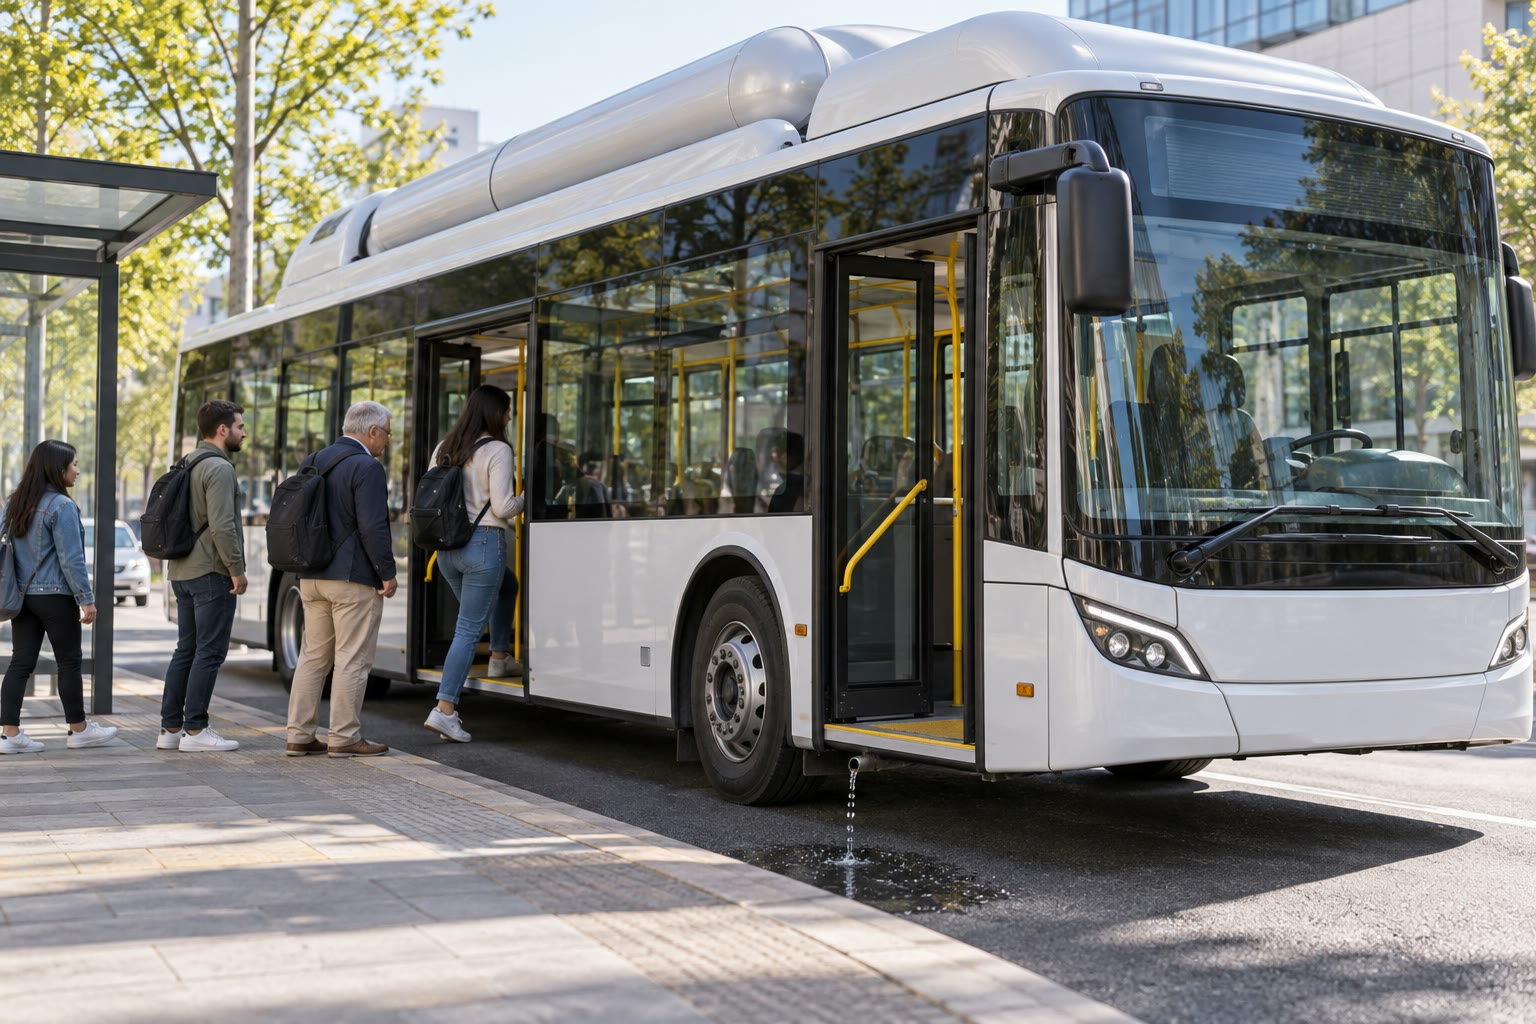
\includegraphics[width=0.62\linewidth]{images/book3/ai/b2-09-fuel-cell-bus.jpg}

{\small Bus sel bahan bakar hidrogen di sebuah halte: tangki-tangki
hidrogennya berada di bawah penutup di atap, dan satu-satunya buangannya
adalah air, yang menetes di bawah bus.}
\end{omfigure}

\section{Kerja listrik dan tetapan Faraday}

\begin{definition}[Tetapan Faraday]\label{def:b2:cell-thermodynamics:faraday}
Yang disebut \emph{tetapan Faraday}\index{tetapan Faraday} adalah muatan
listrik satu mol muatan elementer, $F = N_A e = \qty{96485.33}{C/mol}$.
% ledger: const:F
\end{definition}

\begin{proposition}[Muatan yang mengalir]\label{prop:b2:cell-thermodynamics:charge}
Jika reaksi sebuah sel, yang dituliskan dengan $n$ elektron yang
dipertukarkan, maju sebesar $\Delta\xi$, muatan yang mengalir melalui
rangkaian luar adalah $Q =
nF\,\Delta\xi$.
\end{proposition}

\begin{proof}
Kemajuan $\Delta\xi$ memindahkan $n\,\Delta\xi$ mol elektron dari anode ke
katode melalui kawat, masing-masing dengan muatan sebesar $e$:
$Q = n\,\Delta\xi\,N_A e$.
\end{proof}

Jika muatan $Q$ didorong melalui sebuah rangkaian oleh tegangan $U$, kerja
yang diterima rangkaian adalah $QU$. Dilihat dari sel, yang memberikan
kerja itu, kerja listrik yang diterima sel adalah
$\delta W_{\text{el}} = -U\,\delta Q = -nFU\,
d\xi$.

\begin{omfigure}
\begin{tikzpicture}[font=\small, >={Stealth}]
  \draw[thick, rounded corners, fill=omDef!8] (0,0) rectangle (3.2,2.2);
  \node[align=center] at (1.6,1.1) {sel\\ (sistem)\\ reaksi $d\xi$};
  \draw[->, thick, omThm] (3.2,1.6) -- (5.6,1.6) node[right, align=left] {$\delta W_{\text{el}}$ diberikan\\ $= nFU\,d\xi$};
  \draw[->, thick, omDef] (5.6,0.6) -- (3.2,0.6) node[pos=0, right, align=left] {$\delta Q_{\text{kalor}}$ diterima\\ (tandanya bisa ke dua arah)};
  \draw[<->, thick] (1.6,2.2) -- (1.6,3.0) node[above] {lingkungan pada $T$, $p$};
\end{tikzpicture}

{\small Sel sebagai sistem termodinamika pada suhu dan tekanan tetap: sel
mempertukarkan kalor dengan lingkungannya dan memberikan kerja listrik
melalui rangkaian luar. Dengan konvensi tanda hukum pertama (kerja dan
kalor yang diterima dihitung positif), $\delta W_{\text{el}} = -nFU\,d\xi$.}
\end{omfigure}

\section{Energi Gibbs reaksi sel}

\begin{theorem}[Kerja listrik dan energi Gibbs]\label{thm:b2:cell-thermodynamics:delta-g-nfe}
Sebuah sel yang bekerja pada $T$ dan $p$ tetap memberikan kerja listrik
paling banyak sama dengan penurunan \omterm{def:b2:reaction-free-energy:gibbs-energy}{energi Gibbsnya}: untuk kemajuan
$d\xi$, $nFU\,d\xi \leq -\Delta_r G\,d\xi$. Jika sel itu bekerja secara
reversibel (arus yang infinitesimal), kesamaannya berlaku, dan tegangan sel
adalah gaya gerak listrik
\[
  \Delta_r G = -nFE .
\]
\end{theorem}

\begin{proof}
Hukum pertama pada tekanan tetap, dengan kerja tekanan dipisahkan:
$dH = \delta Q + \delta W_{\text{el}}$. Hukum kedua: $dS \geq \delta Q/T$.
Pada $T$ dan $p$ tetap,
$dG = dH - T\,dS \leq \delta W_{\text{el}} = -nFU\,d\xi$. Dengan
$dG = \Delta_r G\,d\xi$, $\Delta_r G\,d\xi \leq -nFU\,d\xi$, yaitu
$nFU\,d\xi \leq -\Delta_r G\,d\xi$. Untuk perubahan reversibel,
ketaksamaan hukum kedua menjadi kesamaan, dan tegangan yang lalu diukur,
tanpa arus, adalah $E$: $\Delta_r G = -nFE$.
\end{proof}

Jadi sebuah sel hanya dapat berjalan ke arah maju ($d\xi > 0$, sambil
memberikan kerja) jika $\Delta_r G <
0$, yaitu $E > 0$ dengan kutub-kutub
yang dipilih sedemikian rupa sehingga reaksi yang dituliskan berjalan dari
anode ke katode. Sel nyata, yang dilewati arus, memberikan kerja yang lebih
kecil daripada $-\Delta_r G$: selisihnya terdisipasi sebagai kalor di
dalam hambatannya dan pada elektrode-elektrodenya
(\cref{ch:b2:current-potential-curves}).

\begin{example}[Sel Daniell]\label{ex:b2:cell-thermodynamics:daniell}
Untuk \ce{Zn + Cu^2+ -> Zn^2+ + Cu}, $\Delta_r G^\circ = \Delta_f G^\circ(\ce{Zn^2+}) -
\Delta_f G^\circ(\ce{Cu^2+}) = -147.06 - 65.49 = \qty{-212.55}{kJ/mol}$, dan
$n = 2$: $E^\circ = 212\,550/(2 \times 96\,485) = \qty{1.10}{V}$, yaitu
tegangan yang diukur pada sel Daniell dalam kondisi standar.
% ledger: dfg:Zn2+_ao, dfg:Cu2+_ao, const:F, emf:Daniell
\end{example}

\section{Persamaan Nernst dan potensial standar}

Jilid Tahun 1 menerima persamaan Nernst tanpa bukti; kini persamaan itu
diturunkan dari $\Delta_r G = \Delta_r G^\circ + RT\ln Q$.

\begin{theorem}[Persamaan Nernst, diturunkan]\label{thm:b2:cell-thermodynamics:nernst-derived}
Untuk setengah reaksi $\alpha\,\mathrm{Ox} + n\,\mathrm e^- \rightleftharpoons
\beta\,\mathrm{Red}$, potensial elektrode pada suhu $T$ adalah
\[
  E = E^\circ + \frac{RT}{nF}\ln\frac{a_{\mathrm{Ox}}^{\alpha}}{a_{\mathrm{Red}}^{\beta}} ,
\]
dengan aktivitas yang mencakup aktivitas setiap spesies lain dalam
setengah reaksi itu (\ce{H+}, kecuali air), dengan pangkat
stoikiometrinya.
\end{theorem}

\begin{proof}
Potensial sebuah elektrode adalah tegangan sel yang terdiri atas elektrode
hidrogen standar (anode) dan elektrode itu (katode). Reaksinya adalah
\[
  \alpha\,\mathrm{Ox} + \tfrac n2\,\ce{H2} \longrightarrow \beta\,\mathrm{Red} + n\,\ce{H+} ,
\]
yang kuosien reaksinya, dengan $a_{\ce{H+}} = 1$ dan $p_{\ce{H2}} = p^\circ$
pada elektrode hidrogen standar, menjadi $a_{\mathrm{Red}}^\beta/
a_{\mathrm{Ox}}^\alpha$. Dari \cref{thm:b2:cell-thermodynamics:delta-g-nfe},
$E = -\Delta_r G/(nF) = -\Delta_r G^\circ/(nF) - (RT/nF)\ln Q$; dengan
$E^\circ =
-\Delta_r G^\circ/(nF)$, inilah rumusnya. Pada \qty{298.15}{K},
$RT\ln 10/F =
\qty{0.0592}{V}$.
\end{proof}

\begin{proposition}[Potensial standar dari energi Gibbs]\label{prop:b2:cell-thermodynamics:standard-potential}
Dengan konvensi $\Delta_f G^\circ(\ce{H+}, \text{aq}) = 0$ dan
$\Delta_f G^\circ(\ce{H2}, \text{g}) = 0$, potensial standar sebuah pasangan
adalah $E^\circ = -\Delta_r G^\circ/(nF)$, dengan $\Delta_r G^\circ$ \omterm{def:b2:reaction-free-energy:gibbs-energy}{energi
Gibbs} standar setengah reaksi yang dituliskan sebagai reduksi, dan
elektron-elektronnya dianggap berenergi Gibbs nol.
\end{proposition}

\begin{proof}
Dalam reaksi terhadap elektrode hidrogen, $\tfrac n2\,\ce{H2}$ dan
$n\,\ce{H+}$ tidak menyumbang apa pun pada $\Delta_r G^\circ$ menurut
konvensi itu: \omterm{def:b2:reaction-free-energy:gibbs-energy}{energi Gibbs} standar reaksi sel adalah \omterm{def:b2:reaction-free-energy:gibbs-energy}{energi Gibbs} standar
setengah reaksi itu saja.
\end{proof}

\begin{method}[Potensial standar dari tabel]\label{met:b2:cell-thermodynamics:e-from-gibbs}
\begin{enumerate}
  \item Tuliskan setengah reaksi sebagai reduksi, disetarakan dengan
        \ce{H+} dan \ce{H2O}, dengan $n$ elektron.
  \item Hitunglah $\Delta_r G^\circ = \sum\nu_i\Delta_f G^\circ_i$ (produk
        positif), dengan nol untuk unsur-unsur, \ce{H+}, dan elektron.
  \item $E^\circ = -\Delta_r G^\circ/(nF)$, dalam volt dengan
        $\Delta_r G^\circ$ dalam joule per mol.
\end{enumerate}
\end{method}

\begin{example}[Elektrode perak klorida]\label{ex:b2:cell-thermodynamics:agcl}
\ce{AgCl(s) + e- -> Ag(s) + Cl^-}: $\Delta_r G^\circ = -131.228 - (-109.789) =
\qty{-21.439}{kJ/mol}$, $E^\circ = 21\,439/96\,485 = \qty{0.222}{V}$.
Potensialnya hanya bergantung pada aktivitas klorida: dalam larutan
kalium klorida jenuh, elektrode ini merupakan elektrode acuan yang stabil.
% ledger: dfg:Cl-_ao, dfg:AgCl_cr
\end{example}

\begin{proposition}[Menggabungkan potensial]\label{prop:b2:cell-thermodynamics:combining}
Jika setengah reaksi (3), dengan $n_3$ elektron, merupakan jumlah setengah
reaksi (1) dan (2), dengan $n_1$ dan $n_2$ elektron, maka
\[
  n_3E_3^\circ = n_1E_1^\circ + n_2E_2^\circ ;
\]
potensial-potensialnya sendiri tidak dijumlahkan.
\end{proposition}

\begin{proof}
\omterm{def:b2:reaction-free-energy:gibbs-energy}{Energi Gibbs} standar dijumlahkan, $\Delta_r G_3^\circ = \Delta_r G_1^\circ + \Delta_r
G_2^\circ$, dan jumlah elektron dijumlahkan, $n_3 = n_1 + n_2$.
Bagilah setiap $\Delta_r
G^\circ$ dengan $-F$.
\end{proof}

\begin{example}[Besi dalam kedua keadaan oksidasinya]\label{ex:b2:cell-thermodynamics:iron}
\ce{Fe^3+ + e- -> Fe^2+} mempunyai $E^\circ = (-78.90 + 4.7)/(-96.485) = \qty{0.77}{V}$ dan \ce{Fe^2+ + 2e- -> Fe} mempunyai
$E^\circ = -78.90/(2 \times 96.485) =
\qty{-0.41}{V}$. Jadi
\ce{Fe^3+ + 3e- -> Fe}: $E^\circ = (0.77 - 0.82)/3 =
\qty{-0.02}{V}$, bukan
jumlah keduanya.
% ledger: dfg:Fe2+_ao, dfg:Fe3+_ao
\end{example}

\section{Suhu, entropi, dan efisiensi sel bahan bakar}

\begin{definition}[Koefisien suhu]\label{def:b2:cell-thermodynamics:temperature-coefficient}
Yang disebut \emph{koefisien suhu}\index{koefisien suhu} sebuah sel adalah
turunan $(\partial E/\partial T)_p$ gaya gerak listriknya terhadap suhu.
\end{definition}

\begin{proposition}[Entropi dan entalpi dari data sel]\label{prop:b2:cell-thermodynamics:entropy}
Untuk reaksi sel standar,
\[
  \Delta_r S^\circ = nF\,\frac{dE^\circ}{dT}, \qquad
  \Delta_r H^\circ = -nF\Big(E^\circ - T\frac{dE^\circ}{dT}\Big),
\]
dan sel yang bekerja secara reversibel pada suhu $T$ menerima dari
lingkungannya kalor $T\Delta_r S$ per mol reaksi.
\end{proposition}

\begin{proof}
$\Delta_r S^\circ = -d\Delta_r G^\circ/dT$ (dari $dG = -S\,dT + V\,dp$, yang
diturunkan terhadap $\xi$) $= nF\,dE^\circ/dT$; lalu
$\Delta_r H^\circ = \Delta_r G^\circ
+ T\Delta_r S^\circ$. Untuk perubahan
reversibel, $\delta Q = T\,dS = T\Delta_r S\,
d\xi$.
\end{proof}

\begin{method}[Dari data sel ke termodinamika reaksi]\label{met:b2:cell-thermodynamics:cell-data}
\begin{enumerate}
  \item Ukurlah $E$ pada beberapa suhu; kemiringannya adalah $dE/dT$.
  \item $\Delta_r G = -nFE$, $\Delta_r S = nF\,dE/dT$,
        $\Delta_r H = \Delta_r G +
        T\Delta_r S$.
  \item Kalor yang dipertukarkan per mol ketika sel bekerja secara
        reversibel: $T\Delta_r S$; ketika sel memberikan arus pada tegangan
        $U < E$, kalor yang dilepaskan adalah $-\Delta_r H - nFU$ per mol.
\end{enumerate}
\end{method}

Untuk sel hidrogen--oksigen yang menghasilkan air cair, nilai-nilai kunci
CODATA memberikan $\Delta_r H^\circ = \qty{-285.83}{kJ/mol}$ dan
\[
  \Delta_r S^\circ = 69.95 - 130.68 - \tfrac12 \times 205.15 = \qty{-163.3}{J/(K.mol)} ,
\]
sehingga $\Delta_r G^\circ = \qty{-237.14}{kJ/mol}$ dan
$E^\circ = \qty{1.229}{V}$; \omterm{def:b2:cell-thermodynamics:temperature-coefficient}{koefisien suhunya} adalah
$\Delta_r S^\circ/(2F) = \qty{-0.85}{mV/K}$. Sel bahan bakar hidrogen
memberikan tegangan yang lebih kecil dalam keadaan panas daripada dalam
keadaan dingin.
% ledger: dfh:H2O-l, s0:H2O_l, s0:H2_g, s0:O2_g, janafG:H2O_l.298

\begin{omfigure}
\begin{tikzpicture}
\begin{axis}[width=0.48\linewidth, height=5.4cm, xmin=280, xmax=1020,
  ymin=0.95, ymax=1.26, axis x line=bottom, axis y line=left,
  xlabel={$T$ (K)}, ylabel={$E^\circ$ (V)}, tick label style={font=\small},
  label style={font=\small}, title={\small tegangan standar}]
\addplot[omDef, thick, mark=*, mark size=1.2pt] table[x=T, y=E] {figdata/out/bachelor-2-cell-thermodynamics-a-liquid.dat};
\addplot[omThm, thick, mark=*, mark size=1.2pt] table[x=T, y=E] {figdata/out/bachelor-2-cell-thermodynamics-a-gas.dat};
\node[font=\scriptsize, omDef, anchor=north east] at (axis cs:480,1.05) {air cair};
\node[font=\scriptsize, omThm, anchor=south west] at (axis cs:560,1.12) {uap air};
\end{axis}
\end{tikzpicture}\hfill
\begin{tikzpicture}
\begin{axis}[width=0.48\linewidth, height=5.4cm, xmin=280, xmax=1520,
  ymin=0, ymax=1.0, axis x line=bottom, axis y line=left,
  xlabel={$T$ (K)}, ylabel={efisiensi}, tick label style={font=\small},
  label style={font=\small}, title={\small efisiensi maksimum}]
\addplot[omThm, thick, mark=*, mark size=1.2pt] table[x=T, y=eta] {figdata/out/bachelor-2-cell-thermodynamics-b.dat};
\addplot[black!60, thick, dashed] table[x=T, y=eta] {figdata/out/bachelor-2-cell-thermodynamics-b-carnot.dat};
\node[font=\scriptsize, omThm, anchor=south] at (axis cs:700,0.87) {sel bahan bakar};
\node[font=\scriptsize, black!70, anchor=north west] at (axis cs:520,0.40) {Carnot, $T_0 = \qty{298}{K}$};
\end{axis}
\end{tikzpicture}

{\small Sel hidrogen--oksigen menurut tabel JANAF. Kiri: tegangan standar
$-\Delta_r G^\circ/(2F)$ dengan air cair (sampai \qty{500}{K}, dengan
cairan yang dipertahankan dalam keadaan standarnya) dan dengan uap air.
Kanan: efisiensi maksimum $\Delta_r G^\circ/\Delta_r H^\circ$ sel yang
menghasilkan uap, dibandingkan dengan efisiensi Carnot mesin kalor yang
bekerja antara $T$ dan \qty{298}{K}; mesin kalor baru unggul di atas
sekitar \qty{1150}{K}.}
% ledger: janafG:H2O_l.298, janafG:H2O_l.300, janafG:H2O_l.400, janafG:H2O_l.500, janafG:H2O.298, janafG:H2O.300, janafG:H2O.400, janafG:H2O.500, janafG:H2O.600, janafG:H2O.700, janafG:H2O.800, janafG:H2O.900, janafG:H2O.1000, janafdfH:H2O_g.300, janafdfH:H2O_g.400, janafdfH:H2O_g.500, janafdfH:H2O_g.600, janafdfH:H2O_g.700, janafdfH:H2O_g.800, janafdfH:H2O_g.900, janafdfH:H2O_g.1000, janafdfH:H2O_g.1100, janafdfH:H2O_g.1300, janafdfH:H2O_g.1500, janafG:H2O.1100, janafG:H2O.1300, janafG:H2O.1500
\end{omfigure}

\begin{definition}[Efisiensi termodinamik sel bahan bakar]\label{def:b2:cell-thermodynamics:efficiency}
Yang disebut \emph{efisiensi termodinamik}\index{efisiensi termodinamik}
sel bahan bakar adalah rasio kerja listrik yang diberikannya terhadap
kalor yang akan dilepaskan bahan bakarnya melalui pembakaran pada suhu
yang sama, yaitu $-\Delta_r H$ per mol.
\end{definition}

\begin{proposition}[Efisiensi maksimum sel bahan bakar]\label{prop:b2:cell-thermodynamics:efficiency}
\omterm{def:b2:cell-thermodynamics:efficiency}{Efisiensi termodinamik} sel bahan bakar paling besar $\Delta_r G/\Delta_r H$,
yang dicapai ketika sel itu bekerja secara reversibel, dan sama dengan
$(nFU)/(-\Delta_r H)$ pada tegangan kerja $U$. Berbeda dengan mesin kalor,
efisiensi ini tidak dibatasi oleh efisiensi Carnot $1 - T_0/T$.
\end{proposition}

\begin{proof}
Menurut \cref{thm:b2:cell-thermodynamics:delta-g-nfe}, kerja per mol
adalah $nFU \leq
-\Delta_r G$; bagilah dengan $-\Delta_r H$. Sel itu
mengubah energi kimia langsung menjadi kerja pada satu suhu: tidak ada
kalor yang diambil dari sumber panas dan sebagian diberikan kepada sumber
dingin, sehingga batas Carnot, yang menyangkut siklus semacam itu, tidak
berlaku. Batasnya sendiri ditetapkan oleh $T\Delta_r S$, yaitu kalor yang
harus dipertukarkan oleh sel reversibel.
\end{proof}

\begin{omfigure}
\begin{tikzpicture}[font=\small, x=0.022cm, y=0.6cm]
  \draw[->] (0,0) -- (320,0) node[right, font=\scriptsize] {\unit{kJ/mol}};
  \foreach \v in {0,100,200,300} \draw (\v,0) -- (\v,-0.12) node[below, font=\scriptsize] {\v};
  \fill[omThm!70] (0,2.2) rectangle (285.83,2.8);
  \node[anchor=west, font=\scriptsize] at (290,2.5) {$-\Delta_r H^\circ = 285.8$: kalor pembakaran};
  \fill[omDef!70] (0,1.2) rectangle (237.14,1.8);
  \fill[omProp!70] (237.14,1.2) rectangle (285.83,1.8);
  \node[anchor=west, font=\scriptsize] at (290,1.5) {$-\Delta_r G^\circ = 237.1$ kerja $+$ $48.7$ kalor};
  \fill[omDef!40] (0,0.2) rectangle (135.1,0.8);
  \fill[omProp!40] (135.1,0.2) rectangle (285.83,0.8);
  \node[anchor=west, font=\scriptsize] at (290,0.5) {pada \qty{0.70}{V}: $135.1$ kerja $+$ $150.7$ kalor};
\end{tikzpicture}

{\small Ke mana energi satu mol hidrogen pergi dalam sel bahan bakar pada
\qty{298}{K} (air cair). Atas: kalor yang akan dilepaskan oleh nyala.
Tengah: sel reversibel, yang harus melepaskan $-T\Delta_r S^\circ = \qty{48.7}{kJ}$ sebagai kalor apa pun rancangannya. Bawah: sel nyata yang
bekerja pada \qty{0.70}{V}.}
% ledger: dfh:H2O-l, s0:H2O_l, s0:H2_g, s0:O2_g, const:F
\end{omfigure}

\begin{history}[Hukum elektrolisis Faraday]
\begin{minipage}[t]{0.27\linewidth}
\vspace{0pt}
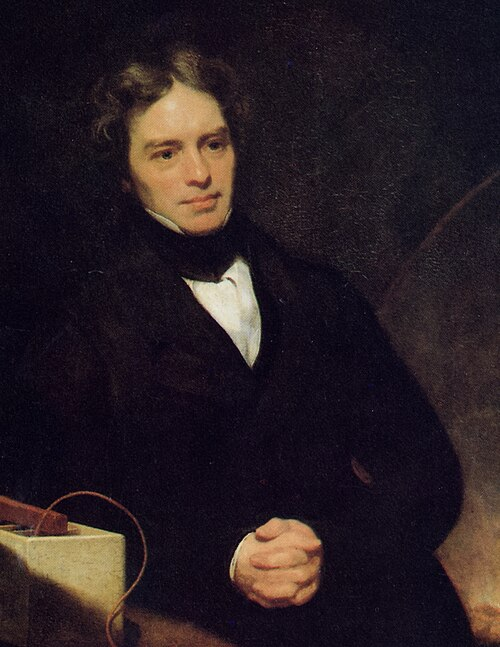
\includegraphics[width=\linewidth]{images/book3/faraday.jpg}
\end{minipage}\hfill
\begin{minipage}[t]{0.69\linewidth}
\vspace{0pt}
Pada tahun 1834 Michael Faraday, yang mengukur hasil-hasil elektrolisis
dengan voltameter rancangannya sendiri, menyatakan bahwa massa zat yang
dihasilkan pada sebuah elektrode sebanding dengan jumlah listrik yang
dialirkan, dan bahwa untuk jumlah listrik tertentu, massa zat-zat yang
berbeda berbanding seperti ekuivalen kimianya. Ia menciptakan kata
elektrode, anode, katode, ion, anion, dan kation. Tetapan yang menyandang
namanya mengubah hukum-hukum itu menjadi $Q = nF\,\Delta\xi$. (Potret oleh
Thomas Phillips, 1842, domain publik, Wikimedia Commons.)
\end{minipage}
\end{history}

\section{Sel konsentrasi}

\begin{definition}[Sel konsentrasi]\label{def:b2:cell-thermodynamics:concentration-cell}
Yang disebut \emph{sel konsentrasi}\index{sel konsentrasi} adalah sel yang
terdiri atas dua setengah sel dari pasangan yang sama, yang hanya berbeda
dalam konsentrasi (atau tekanan) satu spesies.
\end{definition}

\begin{proposition}[Tegangan sel konsentrasi]\label{prop:b2:cell-thermodynamics:concentration-cell}
Dua elektrode logam M yang tercelup dalam larutan \ce{M^{n+}} dengan
konsentrasi $c_1 < c_2$, yang dihubungkan oleh jembatan garam, memberikan
tegangan
\[
  U = \frac{RT}{nF}\ln\frac{c_2}{c_1} ,
\]
dengan kutub positif di sisi yang lebih pekat. Sel itu bekerja sampai
kedua konsentrasi sama.
\end{proposition}

\begin{proof}
Menurut persamaan Nernst, setiap elektrode mempunyai
$E_i = E^\circ + (RT/nF)\ln c_i$ (\omterm{def:b2:chemical-potential:ideal-mixture}{larutan encer ideal}); $E^\circ$ saling
meniadakan dalam selisihnya. Reaksinya adalah \ce{M^{n+}}(sisi 2) $\to$
\ce{M^{n+}}(sisi 1): logam mengendap di sisi yang pekat (katode) dan larut
di sisi yang encer (anode), yang meratakan konsentrasinya;
$\Delta_r G = RT\ln(c_1/c_2) < 0$ sampai keduanya sama.
\end{proof}

\begin{omfigure}
\begin{tikzpicture}[font=\small, >={Stealth}]
  \pic at (0,0) {beaker={0.7}{omDef!10}};
  \pic at (3.6,0) {beaker={0.7}{omDef!32}};
  \pic at (-0.3,0.25) {electrode={black!25}};
  \pic at (3.9,0.25) {electrode={black!25}};
  \pic at (0.35,0.55) {saltbridge={2.9}};
  \pic (m) at (1.8,4.3) {meter={V}};
  % common (black) terminal on the anode side, red (+) on the cathode side
  \fill[black] (1.4,4.03) circle (0.065); \fill[red!70!black] (2.2,4.03) circle (0.065);
  \draw[thick] (-0.15,2.65) |- (m-a);
  \draw[thick] (4.05,2.65) |- (m-b);
  \node[anchor=east] at (-0.95,1.0) {\ce{Ag}};
  \node[anchor=west] at (4.45,1.0) {\ce{Ag}};
  \node at (0.25,-0.35) {\ce{Ag+} \qty{0.010}{mol/L}};
  \node at (3.6,-0.35) {\ce{Ag+} \qty{0.10}{mol/L}};
  \node[anchor=east] at (-0.9,2.3) {$-$ anode};
  \node[anchor=west] at (4.6,2.3) {katode $+$};
  \node[font=\scriptsize] at (-0.1,-0.8) {\ce{Ag -> Ag+ + e-}};
  \node[font=\scriptsize] at (3.7,-0.8) {\ce{Ag+ + e- -> Ag}};
  \node[font=\scriptsize] at (1.8,5.05) {$U = \qty{59}{mV}$};
\end{tikzpicture}

{\small \omterm{def:b2:cell-thermodynamics:concentration-cell}{Sel konsentrasi} perak pada \qty{25}{\degreeCelsius}. Sisi yang encer
adalah anode: perak larut di sana dan mengendap di sisi yang pekat, sampai
kedua konsentrasi sama. $U = 0.0592\log(0.10/0.010) =
\qty{59}{mV}$.}
\end{omfigure}

Prinsip yang sama dipakai untuk mengukur konsentrasi. Elektrode kaca, yang
membran tipisnya memisahkan larutan acuan dari sampel, menghasilkan
potensial membran sebesar $(RT/F)\ln 10 = \qty{59}{mV}$ per satuan
selisih pH pada \qty{25}{\degreeCelsius}: pH-meter dari jilid Tahun 1
adalah \omterm{def:b2:cell-thermodynamics:concentration-cell}{sel konsentrasi} untuk \ce{H+}. Di kedua sisi membran sel hidup,
konsentrasi \ce{K+} yang tidak sama menimbulkan dengan cara yang sama
potensial sebesar beberapa puluh milivolt.

\section{Latihan}

\begin{exercise}[$\star$]\label{exo:b2:cell-thermodynamics:1}
Dari $\Delta_f G^\circ(\ce{H2O}, \text{l}) = \qty{-237.14}{kJ/mol}$,
hitunglah tegangan standar sel hidrogen--oksigen.
\end{exercise}

\begin{exercise}[$\star$]\label{exo:b2:cell-thermodynamics:2}
Sebuah baterai mempunyai kapasitas \qty{1.0}{A.h}. Hitunglah muatan yang
disimpannya, dalam coulomb, dan massa seng yang terkonsumsi di anodenya
(\ce{Zn -> Zn^2+ + 2e-}) ketika baterai itu habis seluruhnya.
\end{exercise}

\begin{exercise}[$\star$]\label{exo:b2:cell-thermodynamics:3}
Sel Daniell memberikan \qty{1.10}{V} tanpa arus. Hitunglah $\Delta_r G$
untuk satu mol seng dan kerja listrik maksimum untuk \qty{10.0}{g} seng.
\end{exercise}

\begin{exercise}[$\star$]\label{exo:b2:cell-thermodynamics:4}
Dua elektrode tembaga tercelup dalam larutan tembaga(II) sulfat
\qty{1.0e-3}{mol/L} dan \qty{0.10}{mol/L}. Hitunglah tegangannya pada
\qty{25}{\degreeCelsius} dan sebutkan kutub-kutubnya.
\end{exercise}

\begin{exercise}[$\star\star$]\label{exo:b2:cell-thermodynamics:5}
Sebuah sel ($n = 2$) mempunyai $E^\circ = \qty{1.015}{V}$ dan
$dE^\circ/dT = \qty{-4.0e-4}{V/K}$ pada \qty{298}{K} (data latihan).
Hitunglah $\Delta_r G^\circ$, $\Delta_r S^\circ$, dan $\Delta_r H^\circ$.
\end{exercise}

\begin{exercise}[$\star\star$]\label{exo:b2:cell-thermodynamics:6}
Sel pada \cref{exo:b2:cell-thermodynamics:5} melepaskan muatan untuk satu
mol reaksi (a) secara reversibel; (b) pada \qty{0.90}{V}. Hitunglah dalam
setiap kasus kerja listrik dan kalor yang dipertukarkan dengan lingkungan.
\end{exercise}

\begin{exercise}[$\star\star$]\label{exo:b2:cell-thermodynamics:7}
Hitunglah $E^\circ(\ce{Fe^3+}/\ce{Fe})$ dari \omterm{def:b2:reaction-free-energy:gibbs-energy}{energi Gibbs} pembentukan
(\ce{Fe^2+} \qty{-78.90}{kJ/mol}, \ce{Fe^3+} \qty{-4.7}{kJ/mol}) lalu
periksalah bahwa nilainya sama dengan $(E_1^\circ + 2E_2^\circ)/3$.
\end{exercise}

\begin{exercise}[$\star\star$]\label{exo:b2:cell-thermodynamics:8}
Hitunglah potensial standar pasangan \ce{AgCl}/\ce{Ag}, lalu potensial
elektrode perak klorida yang tercelup dalam kalium klorida
\qty{0.10}{mol/L}.
\end{exercise}

\begin{exercise}[$\star\star$]\label{exo:b2:cell-thermodynamics:9}
Sel seng--udara memanfaatkan \ce{2Zn + O2 -> 2ZnO}
($\Delta_f G^\circ(\ce{ZnO}) =
\qty{-318.30}{kJ/mol}$). Hitunglah tegangan
standarnya dan energi listrik maksimum, dalam \unit{kW.h}, per kilogram
seng.
\end{exercise}

\begin{exercise}[$\star\star\star$]\label{exo:b2:cell-thermodynamics:10}
Sel bahan bakar metanol langsung menjalankan
\ce{CH3OH(l) + 3/2O2 -> CO2 + 2H2O(l)}. Dari $\Delta_f H^\circ$
(\unit{kJ/mol}): \ce{CH3OH(l)} $-239$, \ce{CO2} $-393.51$, \ce{H2O(l)}
$-285.83$; dan $S^\circ$ (\unit{J/(K.mol)}): \ce{CH3OH(l)} 127.2, \ce{CO2}
213.8, \ce{H2O(l)} 69.95, \ce{O2} 205.15, hitunglah $n$, $E^\circ$, dan
efisiensi maksimumnya.
\end{exercise}

\begin{exercise}[$\star\star\star$]\label{exo:b2:cell-thermodynamics:11}
Sebuah sel ($n = 2$) mempunyai $E = \qty{0.500}{V}$ dan
$dE/dT = \qty{+3.0e-4}{V/K}$ pada \qty{298}{K} (data latihan). Tunjukkan
bahwa, jika bekerja secara reversibel, sel itu memberikan kerja listrik
yang lebih besar daripada $-\Delta_r H$, lalu jelaskan dari mana energi
tambahan itu berasal.
\end{exercise}

\begin{exercise}[$\star\star\star$]\label{exo:b2:cell-thermodynamics:12}
Dua elektrode hidrogen (\qty{1}{bar} \ce{H2}) tercelup dalam larutan acuan
ber-pH 7.00 dan dalam sebuah sampel. Tegangannya \qty{0.177}{V} pada
\qty{25}{\degreeCelsius}, dengan larutan acuan sebagai kutub positif.
Tentukan pH sampel, lalu jelaskan mengapa hasilnya tidak bergantung pada
potensial standar apa pun.
\end{exercise}

\section{Soal: Bus Sel Bahan Bakar}

\begin{problem}[{Soal akhir pekan --- tegangan standar sel
hidrogen--oksigen dari energi Gibbs, koefisien suhunya, efisiensi dan
kalor tumpukan nyata, dan energi dalam satu tangki hidrogen}]
\label{pb:b2:cell-thermodynamics:1}
Sebuah tumpukan sel bahan bakar mempunyai 400 sel yang dipasang seri,
masing-masing dengan membran penukar proton (elektrolit asam). Data pada
\qty{298.15}{K} (CODATA, JANAF): $\Delta_f H^\circ(\ce{H2O}, \text{l}) = \qty{-285.83}{kJ/mol}$, $\Delta_f
G^\circ(\ce{H2O}, \text{l}) = \qty{-237.14}{kJ/mol}$, $\Delta_f G^\circ(\ce{H2O},
\text{g}) = \qty{-228.58}{kJ/mol}$; $S^\circ$ (\unit{J/(K.mol)}): \ce{H2O(l)} 69.95,
\ce{H2} 130.68, \ce{O2} 205.15. $F = \qty{96485}{C/mol}$;
$M(\ce{H2}) =
\qty{2.016}{g/mol}$.
% ledger: dfh:H2O-l, janafG:H2O_l.298, janafG:H2O.298, s0:H2O_l, s0:H2_g, s0:O2_g, const:F, aw:H

\medskip
\noindent\textbf{Bagian I --- Tegangan standar.}
\begin{enumerate}
  \item Tuliskan setengah reaksi di anode dan di katode, serta reaksi
        selnya.
  \item Berapa elektron yang dipertukarkan per molekul hidrogen?
  \item Hitunglah $E^\circ$ jika air terbentuk sebagai cairan.
  \item Hitunglah nilainya jika air keluar sebagai uap.
  \item Jelaskan perbedaannya dengan \omterm{def:b2:reaction-free-energy:gibbs-energy}{energi Gibbs} penguapan air.
  \item Hitunglah $\Delta_r H^\circ$ dan efisiensi maksimum pada
        \qty{298}{K}.
\end{enumerate}

\medskip
\noindent\textbf{Bagian II --- Suhu.}
\begin{enumerate}[resume]
  \item Hitunglah $\Delta_r S^\circ$ untuk air cair.
  \item Simpulkan $dE^\circ/dT$.
  \item Perkirakan $E^\circ$ pada \qty{80}{\degreeCelsius}, suhu kerja
        tumpukan itu.
  \item Bandingkan hasil metode itu dengan nilai JANAF pada \qty{400}{K},
        $\Delta_f
        G^\circ(\ce{H2O}, \text{l}) = \qty{-221.01}{kJ/mol}$.
  \item Berapa kalor yang dipertukarkan sel reversibel per mol hidrogen
        pada \qty{298}{K}? Apakah kalor itu diterima atau dilepaskan?
  \item Perkirakan efisiensi maksimum pada \qty{80}{\degreeCelsius}.
\end{enumerate}

\medskip
\noindent\textbf{Bagian III --- Tumpukan nyata pada \qty{0.70}{V} per sel.}
\begin{enumerate}[resume]
  \item Hitunglah kerja listrik per mol hidrogen.
  \item Hitunglah efisiensi yang diacu pada $\Delta_r H^\circ$ dan pada
        $\Delta_r G^\circ$.
  \item Hitunglah kalor yang dilepaskan per mol hidrogen.
  \item Berapa bagian kalor itu yang tidak dapat dihindari, dan berapa yang
        disebabkan oleh arus?
  \item Tumpukan itu memberikan \qty{300}{A}. Hitunglah konsumsi hidrogen
        satu sel, lalu konsumsi tumpukan, dalam mol dan gram per detik.
  \item Hitunglah daya listrik tumpukan itu.
  \item Hitunglah daya kalor yang harus dibuang oleh sirkuit pendingin.
\end{enumerate}

\medskip
\noindent\textbf{Bagian IV --- Tangki.}
\begin{enumerate}[resume]
  \item Berapa jumlah zat hidrogen dalam \qty{5.0}{kg}?
  \item Berapa muatan yang mengalir melalui sel-sel itu, dihitung untuk
        semuanya, ketika hidrogen ini dioksidasi?
  \item Hitunglah energi listrik yang diberikan oleh tumpukan, dengan
        setiap sel pada \qty{0.70}{V}.
  \item Ubahlah energi itu ke kilowatt-jam.
  \item Berapa lama tumpukan itu dapat memberikan dayanya pada pertanyaan
        18?
  \item Nyatakan energi listrik yang diberikan oleh \qty{5.0}{kg} hidrogen
        pada \qty{0.70}{V} per sel.
\end{enumerate}
\end{problem}
